\documentclass[a4paper,12pt,oneside]{report}
\usepackage[utf8]{vietnam} % Sử dụng tiếng việt
\usepackage[top=2.5cm, bottom=2.5cm, left=3cm, right=2cm] {geometry} % Canh lề trang
\usepackage{graphicx} % Cho phép chèn hỉnh ảnh
\usepackage{placeins}
\usepackage{fancybox} % Tạo khung box
\usepackage{amsthm} % Cho phép thêm các môi trường định nghĩa
\usepackage{latexsym} % Các kí hiệu toán học
\usepackage{amsmath} % Hỗ trợ một số biểu thức toán học
\usepackage{amssymb} % Bổ sung thêm kí hiệu về toán học
\usepackage{amsbsy} % Hỗ trợ các kí hiệu in đậm
\usepackage{times} % Chọn font Time New Romans
\usepackage{sectsty} % Sử dụng để tùy chỉnh kiểu định dạng của tiêu đề
\usepackage{array} % Tạo bảng array
\usepackage{enumitem} % Cho phép thay đổi kí hiệu của list
\usepackage{subfiles} % Chèn các file nhỏ, giúp chia các chapter ra nhiều file hơn
\usepackage{titlesec} % Giúp chỉnh sửa các tiêu đề, đề mục như chương, phần,..
\usepackage{chngcntr} % Dùng để thiết lập lại cách đánh số caption,..
\usepackage{pdflscape} % Đưa các bảng có kích thước đặt theo chiều ngang giấy
\usepackage{afterpage}
\usepackage{capt-of} % Cho phép sử dụng caption lớn đối với landscape page
\usepackage{multirow} % Merge cells
\usepackage{fancyhdr} % Cho phép tùy biến header và footer
\usepackage{enumitem}
\usepackage[natbib,backend=biber,style=ieee]{biblatex} % Giúp chèn tài liệu tham khảo

\usepackage[nonumberlist, nopostdot, nogroupskip]{glossaries}
\usepackage{glossary-superragged}
\setglossarystyle{superraggedheaderborder}
\usepackage{setspace}
\usepackage{parskip}
\usepackage[final]{pdfpages}


\setlength{\glsdescwidth}{9cm}

\bibliography{bibliography/main.bib} % chèn file chứa danh mục tài liệu tham khảo vào

\usepackage{listings}
\usepackage{textcomp}
\usepackage{color}
\usepackage{lstautogobble}

\definecolor{lightgray}{rgb}{.9,.9,.9}
\definecolor{codegreen}{rgb}{0,0.6,0}
\definecolor{codegray}{rgb}{0.5,0.5,0.5}
 
\lstdefinestyle{mystyle}{
    %backgroundcolor=\color{lightgray},   
    commentstyle=\color{codegray},
    keywordstyle=\color{magenta},
    stringstyle=\color{codegreen},
    basicstyle=\scriptsize\ttfamily,
    breakatwhitespace=false,         
    breaklines=true,                 
    captionpos=b,                    
    keepspaces=true,                 
    numbers=none,                
    showspaces=false,                
    showstringspaces=false,
    showtabs=false,             
    tabsize=4,
    upquote=true,
    xleftmargin=1.5\parindent,
    framexleftmargin=3mm,
    inputencoding=utf8,
    autogobble=true,
    frame=single
}

\lstset{style=mystyle} 
 % Phần này cho phép chèn code và formatting code như C, C++, Python

%\makeglossaries
\makenoidxglossaries

% Danh mục thuật ngữ
\newglossaryentry{ml}
{
	name={machine learning},
	description={máy học, học máy}
}

\newglossaryentry{traffic}{
	name = {traffic}, 
	description = {lưu lượng truy cập mạng}
}

\newglossaryentry{ai-gls}{
	name = {artificial intelligence},
	description = {trí tuệ nhân tạo, trí thông minh nhân tạo}
}

\newglossaryentry{entropy}{
	name = {entropy},
	description = {độ hỗn loạn thông tin}
}

\newglossaryentry{information-gain}{
	name = {information gain},
	description = {độ lợi thông tin}
}

\newglossaryentry{supervised-learning}{
	name = {supervised learning},
	description = {học có giám sát}
}

\newglossaryentry{unsupervised-learning}{
	name = {unsupervised learning},
	description = {học không giám sát}
}

\newglossaryentry{regression}
{
	name=regression,
	description={hồi quy}
}

\newglossaryentry{decisiontree}{
	name = {decision tree},
	description = {cây quyết định}
}

\newglossaryentry{bdecisiontree}{
	name = {binary decision tree},
	description = {cây quyết định nhị phân}
}

\newglossaryentry{non-leafnode}{
	name = {non-leaf node},
	description = {nút trong, nút có con}
}

\newglossaryentry{leafnode}{
	name = {leaf node},
	description = {nút lá, nút không có con}
}

\newglossaryentry{childnode}{
	name = {child node},
	description = {nút con}
}

\newglossaryentry{rootnode}{
	name = {root node},
	description = {nút gốc}
}

\newglossaryentry{sibling node}
{
	name={sibling node},
	description={các nút có cùng nút cha}
}

\newglossaryentry{classification}
{
	name=classification,
	description={phân loại}
}

\newglossaryentry{overfitting}{
	name = {overfitting},
	description = {quá khớp}
}

\newglossaryentry{underfitting}{
	name = {underfitting},
	description = {không khớp}
}

\newglossaryentry{accuracy}{
	name = {accuracy},
	description = {độ chính xác}
}

\newglossaryentry{label}{
	name = {label},
	description = {nhãn}
}

\newglossaryentry{normal}{
	name = {normal},
	description = {bình thường}
}

\newglossaryentry{anomalous}{
	name = {anomalous},
	description = {bất thường, dị thường}
}

\newglossaryentry{attribute}{
	name = {attribute},
	description = {thuộc tính}
}

\newglossaryentry{gini}{
	name = {gini index},
	description = {chỉ số đo lường độ không sạch của dữ liệu}
}

\newglossaryentry{request-line}{
	name = {request line},
	description = {chỉ dòng đầu tiên trong gói tin HTTP request}
}

\newglossaryentry{request-body}{
	name = {request body},
	description = {phần nội dung trong gói tin HTTP request}
}

\newglossaryentry{discrete}{
	name = {discrete},
	description = {rời rạc}
}

\newglossaryentry{continuous}{
	name = {continuous},
	description = {liên tục}
}

\newglossaryentry{random-variable}{
	name = {random variable},
	description = {biến ngẫu nhiên}
}

\newglossaryentry{indicatorvariable}{
	name = {indicator variable},
	description = {biến nhị phân}
}

\newglossaryentry{joint-probobability}{
	name = {joint probobability},
	description = {xác xuất hợp}
}

\newglossaryentry{conditional-probability}{
	name = {conditional probability},
	description = {xác suất có điều kiện}
}

\newglossaryentry{training-data}{
	name = {training data},
	description = {dữ liệu huấn luyện}
}

\newglossaryentry{test-data}{
	name = {test data},
	description = {dữ liệu kiểm tra}
}

\newglossaryentry{outcome}{
	name = {outcome},
	description = {đầu ra của dữ liệu}
}

\newglossaryentry{leave-one-out}{
	name = {leave-one-out},
	description = {còn lại một}
}

\newglossaryentry{validation}{
	name = {validation},
	description = {một kĩ thuật để đánh giá độ chính xác của mô hình}
}

\newglossaryentry{cross-validation}{
	name = {cross validation},
	description = {một kĩ thuật để đánh giá độ chính xác của mô hình}
}

\newglossaryentry{train-error}{
	name = {train error},
	description = {mất mát trên dữ liệu huấn luyện}
}

\newglossaryentry{test-error}{
	name = {test error},
	description = {mất mát trên dữ liệu kiểm tra}
}

\newglossaryentry{validation-error}{
	name = {validation error},
	description = {mất mát trên tập đánh giá}
}

\newglossaryentry{validation-set}{
	name = {validation set},
	description = {tập dữ liệu đánh giá}
}

\newglossaryentry{training-score}{
	name = {training score},
	description = {độ chính xác khi huấn luyện}
}

\newglossaryentry{crossvalidation-score}{
	name = {cross-validation score},
	description = {độ chính xác khi dự đoán trên tập kiểm thử}
}


% Danh mục từ viết tắt
% Ví dụ
%\newacronym{http}{HTTP}{HyperText Transfer Protocol}
%\newacronym{ai}{AI}{Artificial Intelligence}
%\newacronym{cart}{CART}{Classification and Regression Trees}
%\newacronym{csdl}{CSDL}{Cơ Sở Dữ Liệu}
%\newacronym{xss}{XSS}{Cross-Site Scripting}
%\newacronym{id3}{ID3}{Iterative Dichotomiser 3}
%\newacronym{csic}{CSIC}{Consejo Superior de Investigaciones Científicas}
\pagestyle{fancy}

\fancyhf{}
\rhead{\footnotesize\nouppercase\rightmark} % Bên phải header: tên section
\lhead{\footnotesize\nouppercase\leftmark} % Bên trái header: tên chapter
\cfoot{\footnotesize\thepage} % Giữa footer: số trang

\setlength{\headheight}{14pt}

\def \TITLE{Báo cáo Đồ án chuyên ngành}
\def \AUTHOR{Nguyễn Trọng Thuỷ}

\newcommand{\titlesize}{\fontsize{18pt}{23pt}\selectfont}
\newcommand{\subtitlesize}{\fontsize{16pt}{21pt}\selectfont}
\titleclass{\part}{top}
\titleformat{\part}[display]
  {\normalfont\huge\bfseries}{\centering}{20pt}{\Huge\centering}
\titlespacing{\part}{0pt}{2em}{1em}
\titlespacing{\section}{0pt}{\parskip}{0.5\parskip}
\titlespacing{\subsection}{0pt}{\parskip}{0.5\parskip}
\titlespacing{\subsubsection}{0pt}{\parskip}{0.5\parskip}


\usepackage[pdftex, % Sử dụng PDF TeX
bookmarks=true, % Tạo bookmarks trong tập tin PDF
colorlinks=false, % Chữ có màu
pdfencoding=auto, % Tự động điều chỉnh encoding của PDF
unicode=true, % Sử dụng Unicode
pdffitwindow=true, % Fit cho vừa cửa sổ
pdfstartview={FitH}, % Zoom file PDF cho vừa khít với nội dung
pdftoolbar=false, % Ẩn đi tool bar trong PDF viewer
pdfmenubar=false % Ẩn đi menu bar trong PDF viewer
]{hyperref}

\hypersetup{pdftitle={\TITLE},
	pdfauthor={\AUTHOR}}

\hypersetup{pdfborder={0 0 0}, citecolor=Black}


\usepackage[all]{hypcap} % Cho phép tham chiếu chính xác đến hình ảnh và bảng biểu

\graphicspath{{figures/}{../figures/}} % Thư mục chứa các hình ảnh

\counterwithin{figure}{chapter} % Đánh số hình ảnh kèm theo chapter. Ví dụ: Hình 1.1, 1.2,..

\title{\bf \TITLE}
\author{\AUTHOR}

\setcounter{secnumdepth}{4} % Cho phép subsubsection trong report
\setcounter{tocdepth}{4} % Chèn subsubsection vào bảng mục lục

\theoremstyle{definition}
\newtheorem{example}{Ví dụ}[chapter] % Định nghĩa môi trường ví dụ

\onehalfspacing
\setlength{\parskip}{6pt}

\begin{document}
\newgeometry{top=2cm, bottom=2cm, left=2cm, right=2cm}
\subfile{cover} % Phần bìa
\restoregeometry

\newgeometry{top=2cm, bottom=2cm, left=2cm, right=2cm}
\subfile{subcover} % Phần bìa
\restoregeometry

\newpage
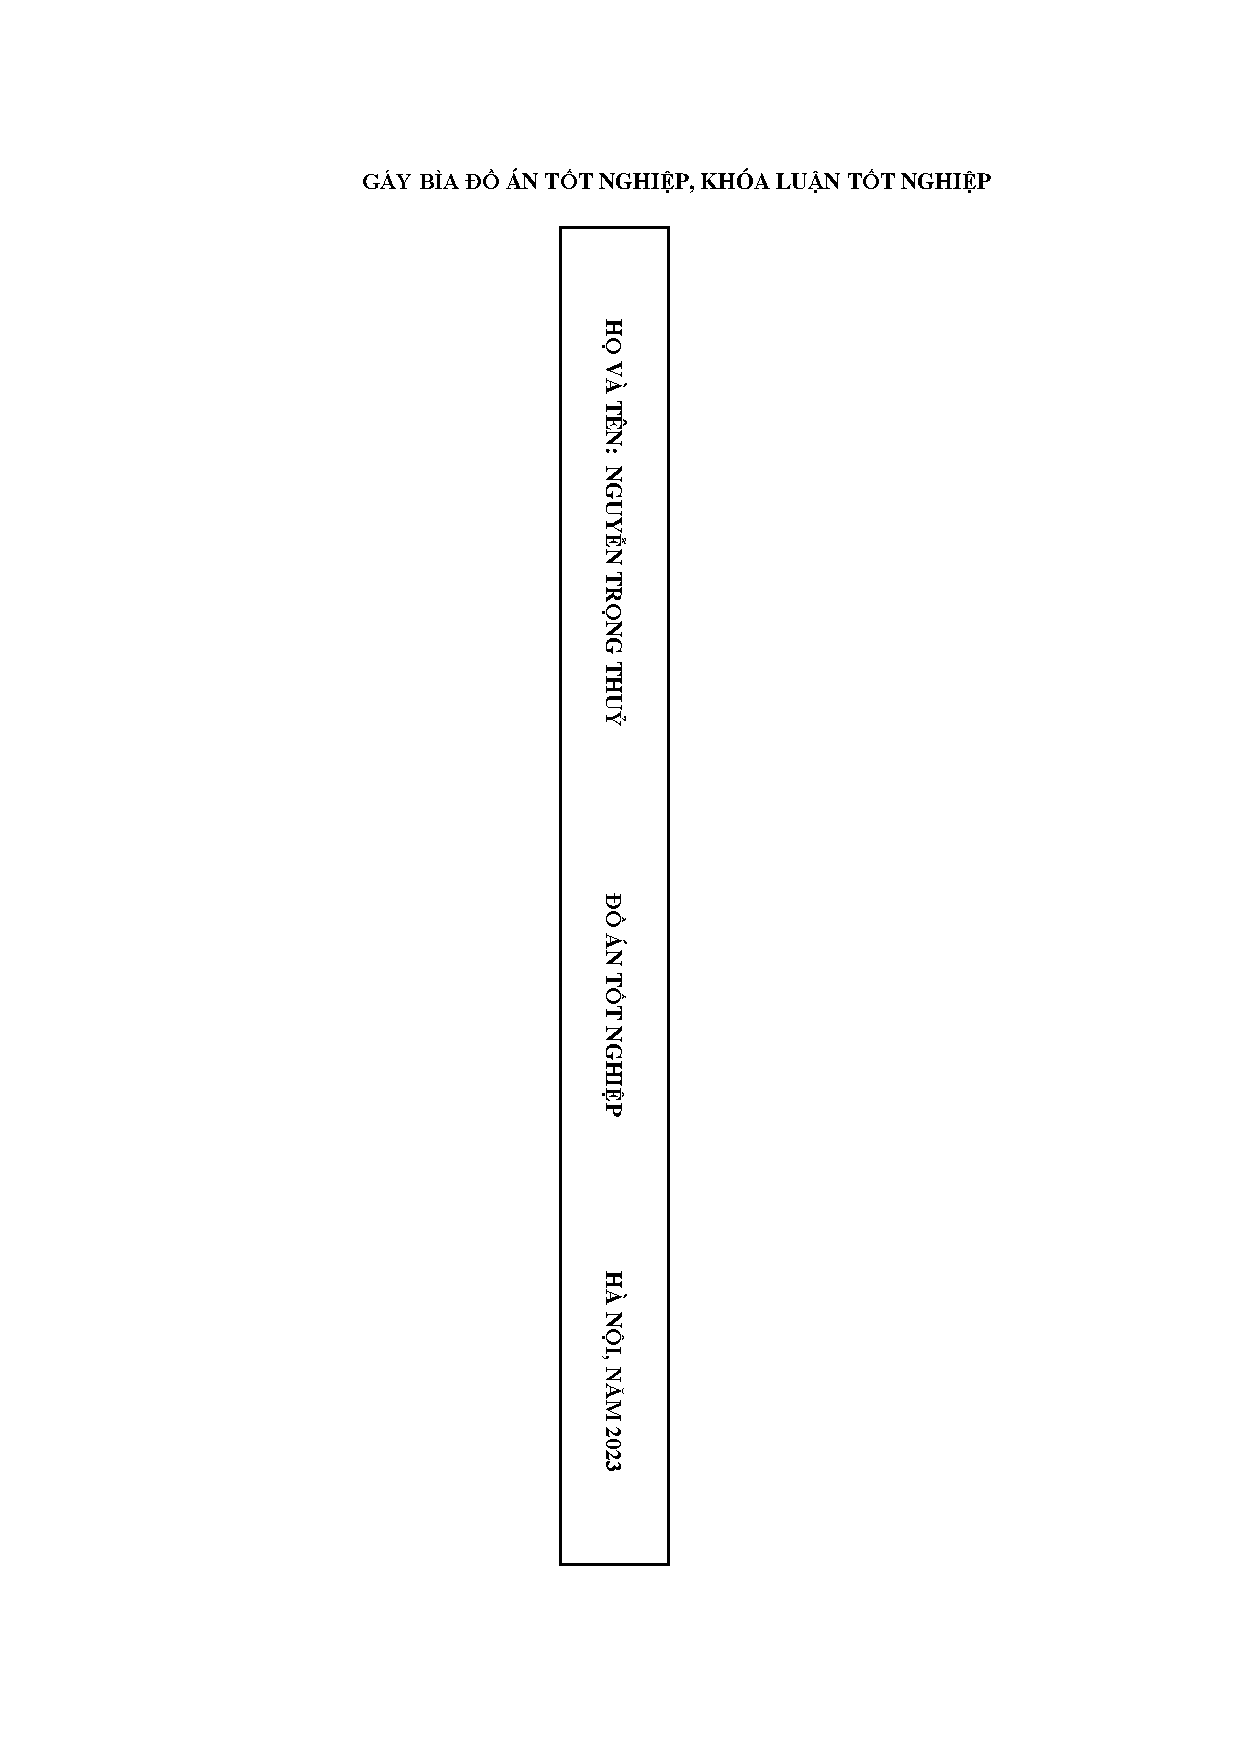
\includepdf[pages=-]{gay-de-cuong.pdf}

\pagenumbering{roman} % Đánh số i, ii, iii, iv, v,..

\section*{\centering{LỜI CAM ĐOAN}}
\addcontentsline{toc}{chapter}{LỜI CAM ĐOAN}
\vspace{15pt}


Tác giả xin cam đoan đây là Đồ án tốt nghiệp của bản thân tác giả. Các kết quả trong Đồ án tốt nghiệp này là trung thực và không sao chép từ bất kỳ một nguồn nào và dưới bất kỳ hình thức nào. Việc tham khảo các nguồn tài liệu (nếu có) đã được thực hiện trích dẫn và ghi nguồn tài liệu tham khảo đúng quy định.
\begin{flushright}
  \textbf{Tác giả Đồ án tốt nghiệp}\\
  \vspace{2cm}
  \textbf{Nguyễn Trọng Thuỷ}
\end{flushright}

\pagestyle{empty} % Header và footer rỗng

\newpage

\section*{\centering{LỜI CẢM ƠN}}
\addcontentsline{toc}{chapter}{LỜI CẢM ƠN}
\vspace{15pt}

Để hoàn thành Đồ án tốt nghiệp với đề tài “Phát triển hệ thống học tập tuỳ chỉnh dựa trên Canvas LMS cho các tổ chức giáo dục đại học”. Trước tiên, tôi xin gửi lời cảm ơn chân thành đến Giáo viên hướng dẫn đồ án Thạc sĩ Kiều Tuấn Dũng và Trường Đại học Thuỷ lợi vì sự hỗ trợ và định hướng quan trọng trong quá trình thực hiện đồ án của tôi.

Giảng viên Kiều Tuấn Dũng đã cung cấp sự chỉ dẫn chuyên môn và hướng dẫn cần thiết để tôi có thể nắm bắt được bối cảnh và phạm vi của đề tài. Nhờ những kiến thức và kinh nghiệm của thầy, tôi đã nhận được sự hỗ trợ và động viên liên tục trong quá trình nghiên cứu và phát triển đề tài.

Tôi cũng muốn bày tỏ lòng biết ơn sâu sắc đến Trường Đại học Thuỷ lợi đã cung cấp cho tôi một môi trường học tập và nghiên cứu thuận lợi.

Tôi rất biết ơn vì sự hỗ trợ và cảm giác được đồng hành trong suốt quá trình thực hiện đồ án của tôi. Sự giúp đỡ và định hướng từ Giáo viên hướng dẫn và Trường Đại học Thuỷ lợi đã góp phần quan trọng vào sự hoàn thiện và thành công của đồ án.

\pagestyle{empty} % Header và footer rỗng
\newpage
\tableofcontents % Mục lục

\listoffigures % Danh sách các hình ảnh
\addcontentsline{toc}{chapter}{Danh mục hình ảnh}

\glsaddall
\newpage
\pagenumbering{arabic}

\newpage
\pagestyle{fancy} % Áp dụng header và footer
\chapter{Tổng quan}
\subfile{chapters/chap1-tong-quan}

\newpage
\pagestyle{fancy} % Áp dụng header và footer
\chapter{Cơ sở lý thuyết và công nghệ}
\subfile{chapters/chap2-co-so-ly-thuyet-va-cong-nghe}

\newpage
\pagestyle{fancy} % Áp dụng header và footer
\chapter{Phân tích yêu cầu}
\subfile{chapters/chap3-phan-tich-yeu-cau}

\newpage
\pagestyle{fancy} % Áp dụng header và footer
\chapter{Xây dựng hệ thống và cài đặt}
\subfile{chapters/chap4-xay-dung-he-thong-va-cai-dat}

\newpage
\pagestyle{fancy} % Áp dụng header và footer
\chapter{Đánh giá và kết luận}
\subfile{chapters/chap5-danh-gia-va-ket-luan.tex}

\newpage
\printbibliography % In ra danh mục tài liệu tham khảo
\addcontentsline{toc}{chapter}{Tài liệu tham khảo}

\renewcommand{\bibname}{Tài liệu tham khảo}
\begin{thebibliography}{9}

  \bibitem{cassandra}
  Apache Software Foundation. (2021). \textit{Apache Cassandra}. Retrieved from \url{https://cassandra.apache.org/}
  
  \bibitem{progit}
  Chacon, S., \& Straub, B. (2014). \textit{Pro Git}. Apress.
  
  \bibitem{react}
  Facebook. (2021). \textit{React - A JavaScript library for building user interfaces}. Retrieved from \url{https://reactjs.org/}
  
  \bibitem{gcp}
  Google Cloud. (2021). \textit{Google Cloud Server}. Retrieved from \url{https://cloud.google.com/}
  
  \bibitem{mailgun}
  Mailgun. (2021). \textit{Mailgun Documentation}. Retrieved from \url{https://documentation.mailgun.com/}
  
  \bibitem{canvaslms}
  Open Source Canvas LMS. (2021). Retrieved from \url{https://github.com/instructure/canvas-lms}
  
  \bibitem{postgresql}
  PostgreSQL. (2021). \textit{PostgreSQL: The world's most advanced open source database}. Retrieved from \url{https://www.postgresql.org/}
  
  \bibitem{html}
  W3Schools. (2021). \textit{HTML Tutorial}. Retrieved from \url{https://www.w3schools.com/html/}
  
  \bibitem{css}
  W3Schools. (2021). \textit{CSS Tutorial}. Retrieved from \url{https://www.w3schools.com/css/}
  
  \bibitem{javascript}
  W3Schools. (2021). \textit{JavaScript Tutorial}. Retrieved from \url{https://www.w3schools.com/js/}
  
\end{thebibliography}
  
\nocite{*} % Tùy chọn cho phép in tất cả danh mục tài liệu tham khảo, kể cả tài liệu không được tham chiếu
\pagestyle{plain}

\end{document}
